%%
	%Information Retrieval & Paper Writing 's Presentation
%%
\documentclass{beamer}
\usepackage{graphicx}
\usepackage{amsmath}
\usepackage{cite} % For citations
\usepackage{hyperref} % For clickable links in the references
\usepackage[absolute,overlay]{textpos}
\usepackage{tikz}

\mode<presentation>
{
\usetheme{Madrid}
\usecolortheme{default}
}

%Change the reference icon to a standard format
\setbeamertemplate{bibliography item}[text]

%------TITLE PAGE------
\title[Big Data]{Unveiling the Power of Big Data}
\subtitle{Transforming Insights through Data Science on Big Data Platforms}
\author[Authors]{Zhanbo Hua \and Xiangrui Zhao \and Haozhe Zhou \and Haopo Zhang}
\institute[CUMT]{School of Computer Science \& Technology\\China University of Mining and Technology}
\date{September 20, 2023}

\iffalse
%------Highlight the title of the current section------
\AtBeginSection[]
{
	\begin{frame}
		\frametitle{Table of Contents}
		\tableofcontents[currentsection]
	\end{frame}
}
\fi


\begin{document}

% Logo at the top center
\begin{textblock*}{5cm}(5.7cm,0.1cm) % Adjust the position as needed

\includegraphics[width=1.5cm]{resources/logo0.png}
\end{textblock*}

%insert title page
\frame{\titlepage}

\makeatletter
\setbeamertemplate{footline}{
  \ifnum\c@framenumber>1%
    \tikz[remember picture,overlay]{
      \node at (current page.north east) [anchor=north east, yshift=-0.2cm] {
\includegraphics[width=5cm]{resources/logo1.png}};
    }
  \fi
}
\makeatother

%insert contents
\begin{frame}
	\frametitle{Table of Contents}
	\tableofcontents
\end{frame}

%Introduction
\section{Introduction}
	%Frame0
	\begin{frame}
	\frametitle{Introduction}
		\begin{itemize}
  			\item Big Data is transforming industries worldwide.
  			\item In this presentation, we explore its significance and applications.
  			\item Let's begin our journey into the world of Big Data.
		\end{itemize}
	\end{frame}
	%Frame1
	\begin{frame}[label=definition]{Introduction}
	\framesubtitle{Definition}
		\begin{columns}
    		\begin{column}{0.5\textwidth} % Adjust the width as needed
      		\textbf{Big Data Definition:}
      		\begin{itemize}
        		\item Big Data refers to extremely large and complex datasets that cannot be easily managed, processed, or analyzed using traditional data processing tools.
        		\item It is characterized by the four Vs: Volume, Velocity, Variety, and Veracity.
      		\end{itemize}
    		\end{column}
    		\begin{column}{0.5\textwidth} % Adjust the width as needed
      		\begin{figure}
        		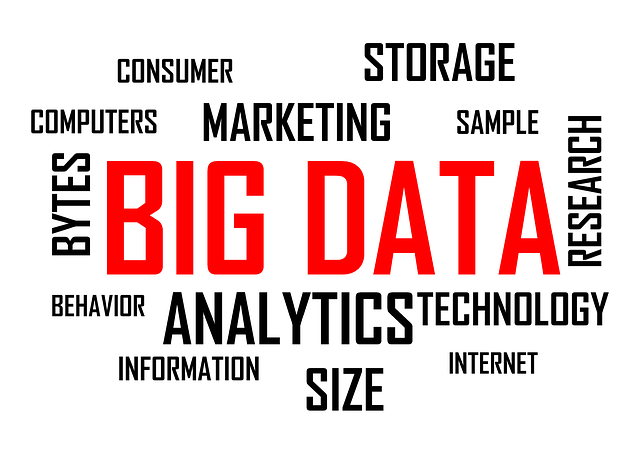
\includegraphics[width=\linewidth]{resources/bigdata0.png} % Adjust the path and size of the image
        		\caption{Big Data}
      		\end{figure}
    		\end{column}
  		\end{columns}
	\end{frame}
	%Frame2
	\begin{frame}[label=definition]{Introduction}
	\framesubtitle{Big Data is all around us}
		\begin{columns}
			\begin{column}{0.5\textwidth} % Adjust the width as needed
      		\begin{figure}
        		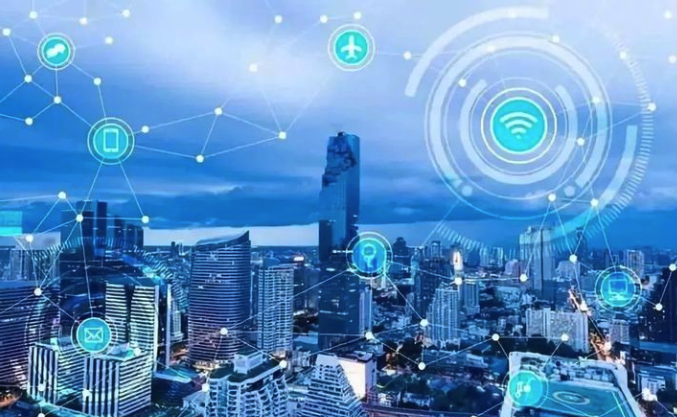
\includegraphics[width=\linewidth]{resources/bigdata1.png} % Adjust the path and size of the image
        		\caption{Data Generation}
      		\end{figure}
    		\end{column}
    		\begin{column}{0.5\textwidth} % Adjust the width as needed
      		\textbf{Data is generated all the time:}
      		\begin{itemize}
        		\item The Internet of Things, cloud computing, mobile Internet, mobile phones and tablets, PCs, and various sensors everywhere are all sources or carriers of big data.
        		\item It can be said that big data is all around us, producing and carrying large amounts of data every day.
      		\end{itemize}
    		\end{column}
		\end{columns}
	\end{frame}
	
%Data Science in Big Data
\section{Data Science in Big Data}
	\begin{frame}
	\frametitle{Data Science in Big Data}
		\begin{columns}
			\begin{column}{0.5\textwidth}
				\begin{itemize}
  					\item Data Science is the key to unlocking insights from Big Data.
  					\item It involves data collection, analysis, and interpretation.
  					\item Data Science helps organizations make data-driven decisions.
				\end{itemize}
			\end{column}
			\begin{column}{0.5\textwidth}
				\begin{figure}
        		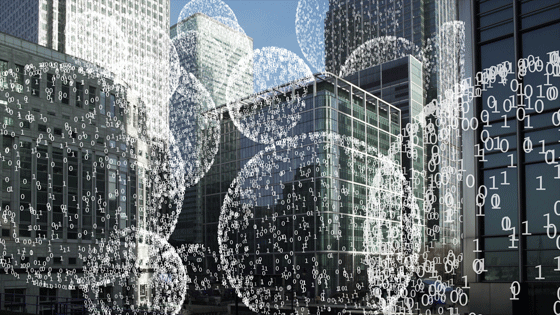
\includegraphics[width=\linewidth]{resources/bigdata2.png} % Adjust the path and size of the image
        		\caption{Data Science}
      			\end{figure}
			\end{column}
		\end{columns}
	\end{frame}

%Case Studies
\section{Case Studies}
	%Frame0
	\begin{frame}
	\frametitle{Case Studies}
		\begin{itemize}
  			\item Let's explore real-world examples to understand the impact of Big Data and Data Science.
  			\item Case Study 1: E-commerce Personalization
  			\item Case Study 2: Healthcare Analytics
		\end{itemize}
	\end{frame}
	%Frame1
	\begin{frame}
	\frametitle{Case Studies}
	\framesubtitle{E-commerce Personalization}
		\begin{columns}
			\begin{column}{0.5\textwidth}
				\textbf{Personalization features on business-to-consumer e-commerce:}
				\begin{itemize}
  					\item The rapid growth of technology and social media enables easy real-time information exchange and interaction among users, impacting online personalized advertising performance. However, it also poses challenges in terms of consumer trust and privacy concerns for researchers.
				\end{itemize}
			\end{column}
			\begin{column}{0.5\textwidth}
				\begin{figure}
        		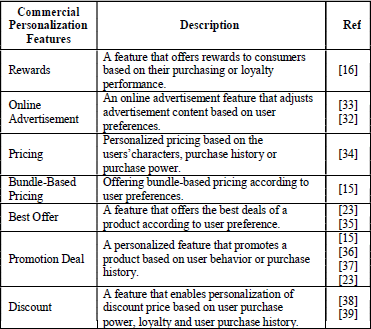
\includegraphics[width=\linewidth]{resources/CommercialPersonalization.png} % Adjust the path and size of the image
        		\caption{Commercial personalization features}
      			\end{figure}
			\end{column}
		\end{columns}
	\end{frame}
	%Frame2
	\begin{frame}
	\frametitle{Case Studies}
	\framesubtitle{Healthcare Analytics}
		\begin{columns}
			\begin{column}{0.5\textwidth} % Adjust the width as needed
      		\begin{figure}
        		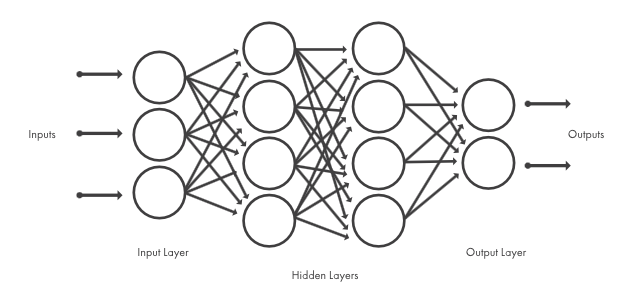
\includegraphics[width=\linewidth]{resources/deeplearning.png} % Adjust the path and size of the image
        		\caption{Neural networks}
      		\end{figure}
    		\end{column}
    		\begin{column}{0.5\textwidth} % Adjust the width as needed
      		\textbf{Applying data science to healthcare data:}
      		\begin{itemize}
        		\item Coronavirus disease 2019 (COVID-19) data are notable healthcare data. The disease broke out in 2019, was declared as a pandemic on 11 March 2020, and is still prevailing more than two years later (in 2022). Healthcare informatics on COVID-19 data helps get a better understanding of the disease and find ways to prevent or combat it.
      		\end{itemize}
    		\end{column}
		\end{columns}
	\end{frame}
	
%Challenges and Limitations
\section{Challenges and Limitations}
	\begin{frame}
	\frametitle{Challenges and Limitations}
		\begin{itemize}
  			\item While Big Data offers immense potential, it comes with challenges and limitations:
  			\item Challenge 1: Data Privacy and Security
  			\item Challenge 2: Scalability
  			\item Limitation 1: Representativeness: a complete sample is never possible
  			\item Limitation 2: Timeliness: Second-level value exists
  			\item We must address these challenges to harness the full power of Big Data.
		\end{itemize}
	\end{frame}
	
%Future Trends
\section{Future Trends}
	\begin{frame}
	\frametitle{Future Trends}
		\begin{columns}
			\begin{column}{0.5\textwidth}
				\begin{itemize}
  					\item The world of Big Data is constantly evolving.
  					\item Future trends include:
  					\item Trend 1: Edge Computing
  					\item Trend 2: AI and Machine Learning Integration
  					\item Trend 3: Advancements in Big Data Platforms
  					\item Stay updated to stay competitive in the era of Big Data.
				\end{itemize}
			\end{column}
			\begin{column}{0.5\textwidth}
				\begin{figure}
        		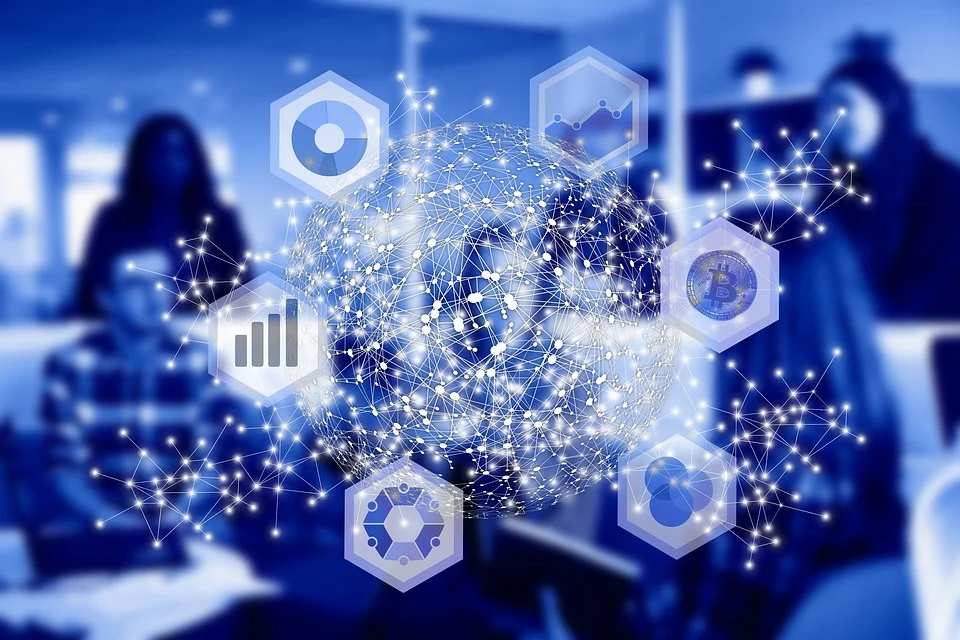
\includegraphics[width=\linewidth]{resources/fituretrends.png} % Adjust the path and size of the image
        		\caption{Future Trends}
      			\end{figure}
			\end{column}
		\end{columns}
	\end{frame}

%Conclusion
\section{Conclusion}
	\begin{frame}
	\frametitle{Conclusion}
		\begin{minipage}[c][0.4\textheight][c]{\linewidth}
			\centering
			\begin{itemize}
  				\item Big Data, Data Science, and Data Mining are revolutionizing industries.
  				\item With the right strategies, organizations can harness Big Data's power.
  				\item Embrace the future of data for informed decision-making.
			\end{itemize}
		\end{minipage}
		\begin{minipage}[c][0.4\textheight][c]{\linewidth}
			\centering
			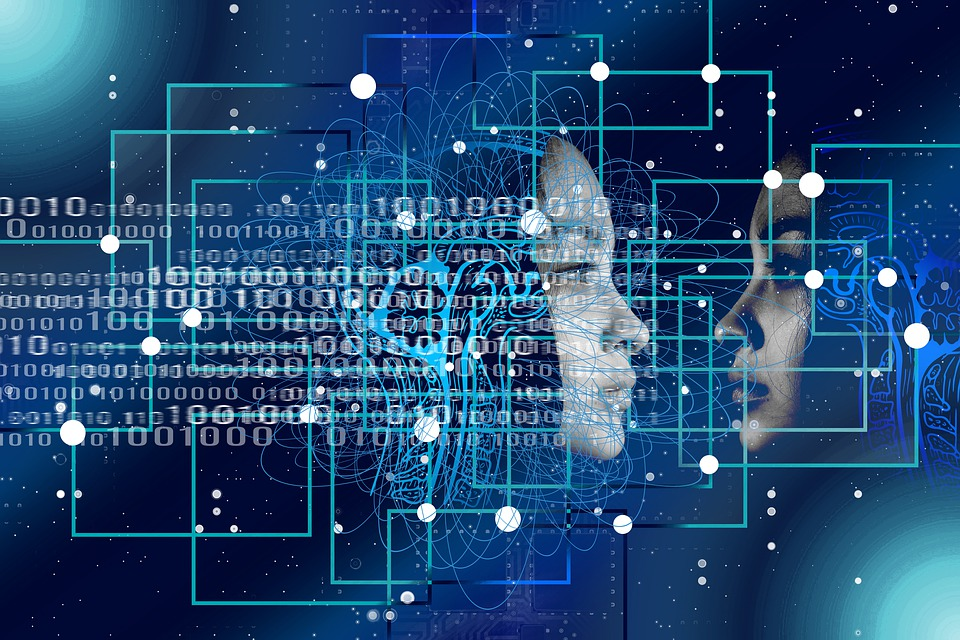
\includegraphics[width=0.5\linewidth]{resources/end.jpeg}
		\end{minipage}
	\end{frame}
	
%References
\section{References}
	\begin{frame}[label=references]{References}
		\begin{thebibliography}{9}
			\bibitem{chen2014}
			Chen, J., Song, L., Liu, X., \& Wang, L. (2014). Big Data Deep Learning: Challenges and Perspectives. IEEE Access, 2, 514-525.
			\bibitem{provost2013}
			Provost, F., \& Fawcett, T. (2013). Data Science for Business: What You Need to Know about Data Mining and Data-Analytic Thinking. O'Reilly Media.
			\bibitem{zikopoulos2012}
			Zikopoulos, P., Eaton, C., deRoos, D., Deutsch, T., Lapis, G., \& Deroos, D. (2012). Understanding Big Data: Analytics for Enterprise Class Hadoop and Streaming Data. McGraw-Hill Osborne Media.
			\bibitem{ghemawat2003}
			Ghemawat, S., Gobioff, H., \& Leung, S. T. (2003). The Google file system. ACM SIGOPS Operating Systems Review, 37(5), 29-43.
			\bibitem{white2015}
			White, T. (2015). Hadoop: The Definitive Guide. O'Reilly Media.
			\bibitem{manyika2011}
			Manyika, J., Chui, M., Brown, B., Bughin, J., Dobbs, R., Roxburgh, C., \& Byers, A. H. (2011). Big Data: The Next Frontier for Innovation, Competition, and Productivity. McKinsey Global Institute.
		\end{thebibliography}
	\end{frame}

\end{document}
